% proci.tex

\cleardoublepage
\chapter{LODESTAR}\label{chapter:LODESTAR}	
This chapter covers the package LODESTAR (Launch Optimisation and Data Evaluation for Scramjet Trajectory Analysis Research), which has been used to calculate the optimal trajectories of the rocket-scramjet-rocket system. The structure of LODESTAR is presented, as well as the set-up of LODESTAR for the rocket-scramjet-rocket trajectory optimisation, and the verification methods used to determine if a solution has converged correctly.

LODESTAR optimises a trajectory towards a user-defined objective function, such as maximum payload-to-orbit, subject to constraints which bound the operational region of a vehicle.
LODESTAR is MATLAB based and utilises GPOPS-2[CITEXX], a proprietary pseudospectral method optimisation package which utilises an hp-adaptive version of the Radau pseudospectral method, ie. the pseudospectral method with collocation at Legendre-Gauss-Radau points. At these points, the derivatives of the approximating polynomials are constrained to the vehicle dynamics. Between these points, the Legendre polynomials used for approximation ensure that the dynamics of the launch vehicles are interpolated accurately. The operation of the pseudospectral method is described in further detail in Section \ref{sec:Propulsion}.
LODESTAR provides setup files to configure GPOPS-2 for multiple vehicle launch optimisation, and processing functions to asses the viability of the optimised solutions and plot the solutions effectively. 
LODESTAR also provides simulations of the vehicles within the launch system including interpolation schemes specifically designed to provide smooth, continuous aerodynamic and engine properties to ensure that the optimisation converges correctly. 
 Both rocket-powered and scramjet-powered vehicles are accurately modelled within LODESTAR in 6 degrees of freedom. LODESTAR contains multiple modes configured for the SPARTAN launch system, which are able to optimise trajectories for,
\begin{enumerate}
	\item The ascent of the first stage rocket,
	\item The ascent of the second stage scramjet-powered accelerator,
	\item The flyback of the second stage scramjet-powered accelerator,
	\item The ascent of the third stage rocket, and
	\item Combined trajectories of multiple stages in any combination.
\end{enumerate}
 
 


Figure \ref{fig:FlowChartSmall} illustrates a simplified iteration of the pseudospectral solver. GPOPS-2 provides an initial guess of the solution to the external modules, over an initial mesh of nodes.
The external modules calculate the aerodynamic and engine performance of the launch system at each point along the trajectory, along with atmospheric conditions. This data is then used to calculate the dynamics of the vehicle along the trajectory. The constraints and cost function are then evaluated by GPOPS-2 and passed through to the IPOPT nonlinear optimisation package\cite{Wachter2006}, which updates the guess of the state and control variables. This process is repeated for a set number of iterations, with the solution evaluated at each iteration to compute the feasibility and optimality of the solution. This process repeats until the solver reaches a predefined tolerance of optimality, or a predefined number of iterations. At this point, GPOPS-2 updates the node mesh, clustering nodes and creating mesh segments around key sections of the trajectory to improve accuracy. The process repeats for a number of mesh iterations defined by the user. 
\begin{figure}[ht]
	\centering
	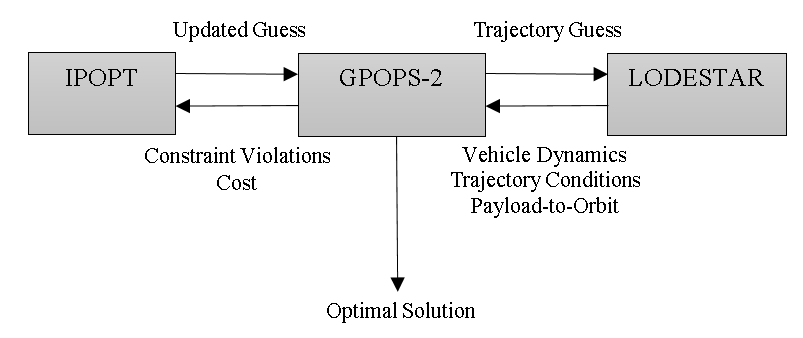
\includegraphics[width=0.75\linewidth]{figures/4_LODESTAR/FlowChartSmall}
	\caption{The optimisation process.}
	\label{fig:FlowChartSmall}
\end{figure}

Due to the nature of the pseudospectral method, it is possible that GPOPS-2 will not be able to converge to a physically valid or optimal solution. 
LODESTAR contains a number of verification modules which assess the optimised trajectory solution to ensure that the solution has converged sufficiently, and that the dynamics of the solution are accurate. 
To aid in ensuring that an optimal solution is reached, GPOPS-2 is initiated from four separate initial guesses, with final altitude guess varied by 1km between each guess. These iterations of GPOPS-2 are run in parallel, using Matlab's Parfor function. After all iterations of GPOPS-2 have completed, the state feasibility is calculated for each solution. The 'best' solution is chosen as the solution with the most accurately modelled dynamics. 



\section{Vehicle Simulation}


Each of the vehicles within the rocket-scramjet-rocket launch system are simulated by establishing a set of dynamic equations which fully describe the motion of the vehicle in terms of the time, states ($\mathbf{x}$), and controls ($\mathbf{u}$) of the system;
\begin{equation}
\dot{\textbf{x}}(t) = f[t,\textbf{x}(t),\textbf{u}(t)].
\end{equation}
 The states and controls are the variables which define the time dependent physical characteristics of the system. The state variables are dependent on the controls and the system dynamics, while the control variables are the variables which drive the behaviour of the system and are independently variable.  
 
These dynamic equations consist of the equations of motion of the vehicle, as well as other important time varying parameters, such as fuel mass flow rate. 
The dynamic equations are defined by the coordinate system, and the outputs of each vehicle model. These are nonlinear equations which depend on the interpolation of data sets which supply the atmospheric, aerodynamic and propulsion characteristics of each vehicle. 
The methods used to interpolate these data sets must be as smooth and continuous as possible, and cover the entire possible operational range of the vehicle. 
Even if the solution is well within the range of all input data sets, the solver will potentially explore all regions within the user defined bounds. 
If there are large discontinuities or inaccurate extrapolation effects within the possible solution space, the solver may be unable to converge, or converge to a physically invalid solution. 


\subsection{6DOF Equations of Motion}


The dynamics of the vehicle are calculated in six degrees of freedom, illustrated in Figures \ref{fig:global} and \ref{fig:Axes}, with yaw constrained to zero. 
The dynamics of all stages are calculated using an geodetic rotational reference frame, written in terms of the angle of attack $\alpha$, bank angle $\eta$, radius from centre of Earth $r$, longitude $\xi$, latitude $\phi$, flight path angle $\gamma$, velocity $v$ and heading angle $\zeta$. The equations of motion are given from \cite{Josselyn2002a}:
\begin{figure}[ht]
	\centering
	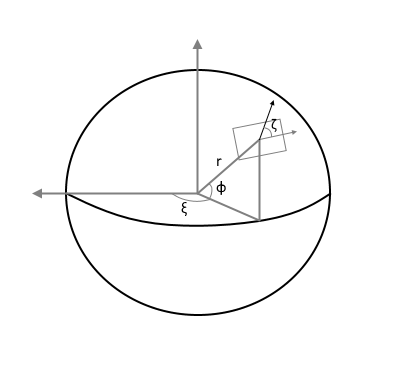
\includegraphics[width=0.7\linewidth]{figures/4_LODESTAR/global}
	\caption{The Earth-fixed components of the geodetic rotational coordinate system.}
	\label{fig:global}
\end{figure}
\begin{figure}[ht]
	\centering
	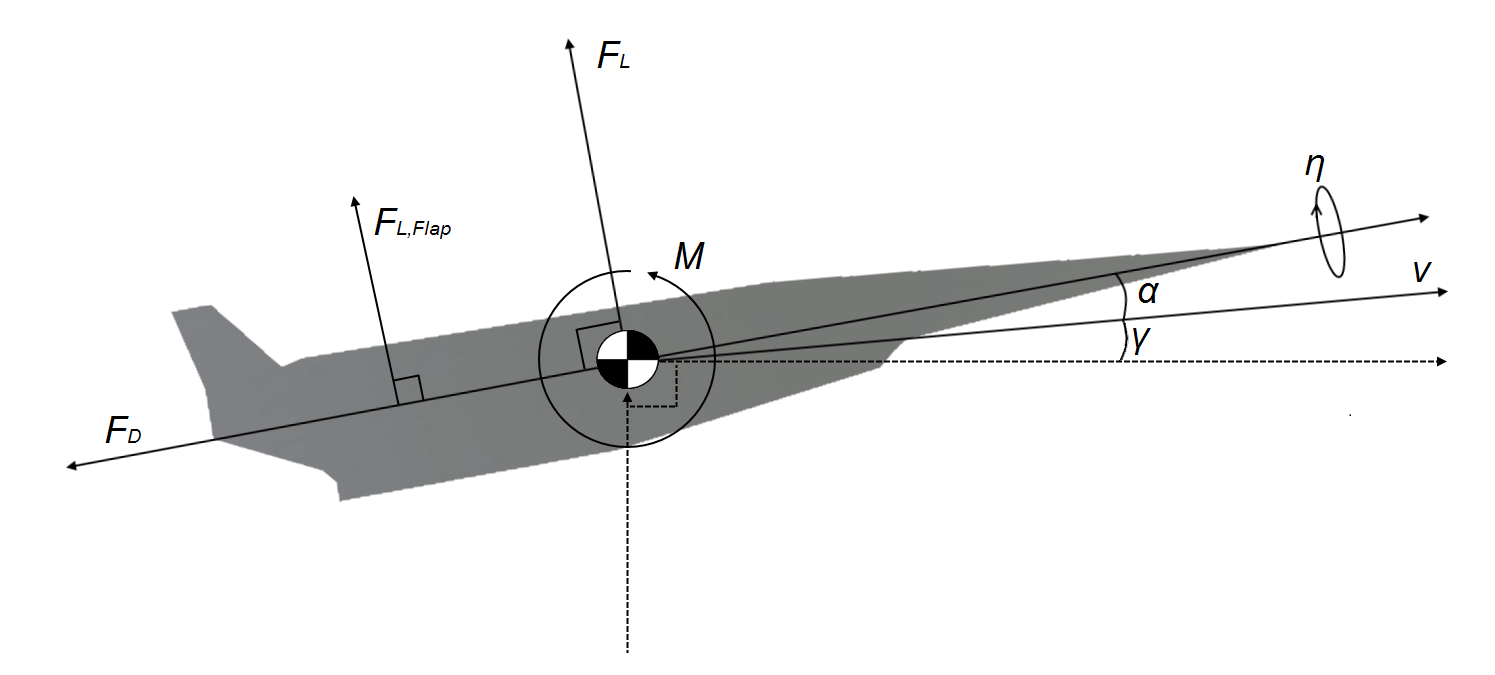
\includegraphics[width=0.9\linewidth]{figures/4_LODESTAR/Axes}
	\caption{The vehicle-based components of the coordinate system.}
	\label{fig:Axes}
\end{figure}


\begin{equation}
\dot{r} = v \sin \gamma
\end{equation}

\begin{equation}
\dot{\xi} = \frac{v\cos \gamma \cos \zeta}{r \cos \phi}
\end{equation}

\begin{equation}
\dot{\phi} = \frac{v\cos\gamma\sin\zeta}{r}
\end{equation}
\begin{equation}
\dot{\gamma} = \frac{T\sin\alpha \cos\eta}{mv} + (\frac{v}{r}-\frac{\mu_E}{r^2 v})\cos\gamma + \frac{L}{mv}
+ \cos\phi[2\omega_E \cos\zeta + \frac{\omega_E^2 r}{v}(\cos\phi\cos\gamma+\sin\phi\sin\gamma\sin\zeta)]
\end{equation}
\begin{equation}
\dot{v} = \frac{T\cos\alpha}{m}-\frac{\mu_E}{r^2}\sin\gamma - \frac{D}{m}
+ \omega_E^2 r\cos\phi(\cos\phi\sin\gamma-\sin\phi\cos\gamma\sin\zeta)
\end{equation}
\begin{equation}\label{eq:heading}
\dot{\zeta} = \frac{T\sin\alpha \sin\eta}{mv \cos \gamma}-\frac{v}{r}\tan\phi\cos\gamma\cos\zeta +2\omega_E\cos\phi\tan\gamma\sin\zeta - \frac{\omega_E^2 r}{v\cos\gamma}\sin\phi\cos\phi\cos\zeta-2\omega_E\sin\phi 
\end{equation}



\section{Mission Definition}
LODESTAR has been developed to be able to simulate any mission desired of the rocket-scramjet-rocket launch system. However, the configuration of the optimal control routines must be tailored towards the specific mission profile desired.
The mission chosen for the optimal trajectory calculation is a launch to sun synchronous orbit. 
A satellite in sun synchronous orbit is close to polar inclination, regressing so that it keeps its orbital alignment to the sun. The sun synchronous is one of the most commonly used types of orbit for space science missions, as it has many useful properties\cite{Boain2004}. A sun synchonous orbit allows for global coverage, passing over each latitude at the same time each day, illustrated in Figure \ref{fig:SSO}. It also allows for a satellite to either have full sun and have consistent power generation, or alternatively, allows for a satellite to have a consistent 'dark side' each day to alleviate thermal issues\cite{Boain2004}. A sun synchronous orbit at 566km has been used in previous studies as the target orbit\cite{Preller2017b}, and this orbit is also used for the current work. 
\begin{figure}[ht]
\centering
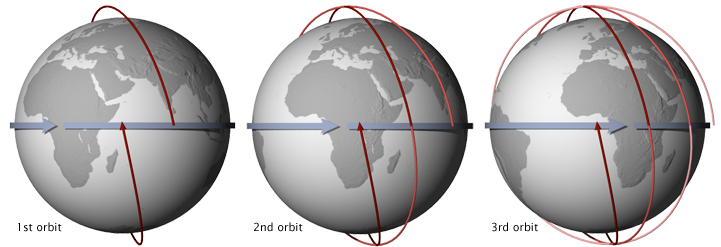
\includegraphics[width=0.8\linewidth]{figures/4_LODESTAR/SSO}
\caption{Sun synchronous orbit illustration, passing over the equator at the same time each day\cite{NASASSO}.}
\label{fig:SSO}
\end{figure}

The launch site selected for the simulation is the proposed Equatorial Launch Australia launch site near Nhulunbuy in the Northern Territory, Australia[CITEXX]. This proposed launch site looks to take advantage of the remoteness of northern Australia, as well as its close proximity to the equator. While the proximity to the equator of this launch site is slightly disadvantageous for launch to sun synchronous orbits, the possibility of launch directions from this location, and its active development, make it an appropriate choice as a practical launch location within Australia. The site is 'about 30km south of Nhulunbuy'[CITEXX news.com.au] which places it within the approximate region indicated in Figure \ref{fig:SiteLocation}.

\begin{figure}[ht]
\centering
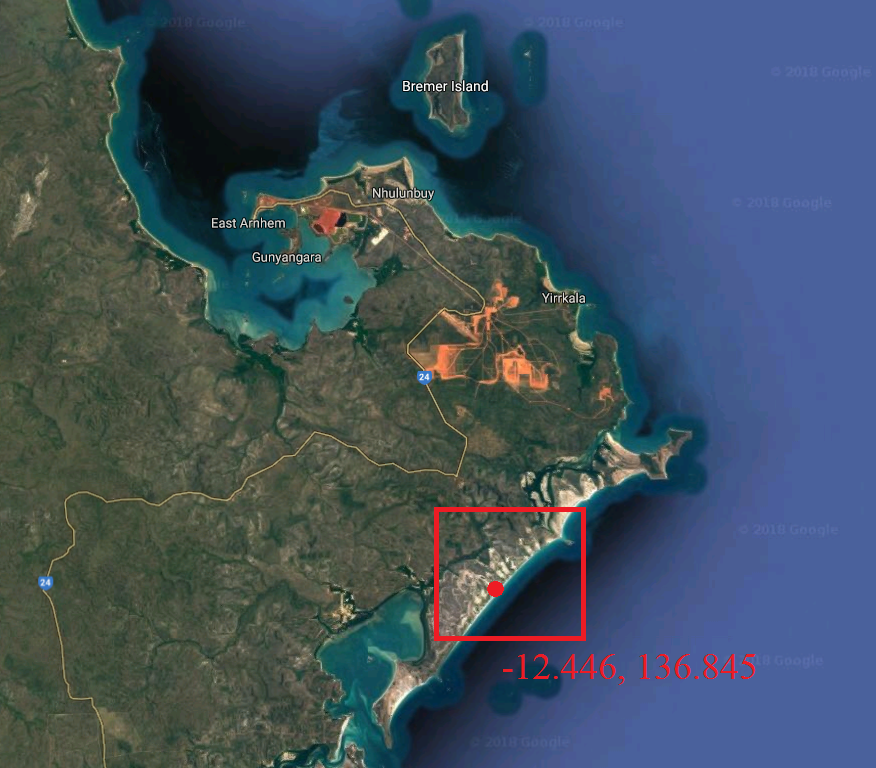
\includegraphics[width=0.7\linewidth]{figures/4_LODESTAR/SiteLocation}
\caption{Approximate location of the ELA launch site. Image from Google maps.}
\label{fig:SiteLocation}
\end{figure}


\section{Optimal Control Problem Structure}

The pseudospectral method used by GPOPS-2 is described in detail in section \ref{sec:Optimisation}. Practically, the implementation of optimal control involves the specification of the dynamics of the system to be optimised, as well as the set of constraints and objectives that define the optimisation problem. 
 Together, these define the optimisation problem being solved.

\noindent \textit{Cost Function}

\noindent The cost function, $J$, defines the target of the optimisation problem. 
This cost function may be any function which is defined by the states or controls of the optimisation problem. The cost function is defined as follows:
\begin{equation} \label{eq:cost}
J(t,\textbf{x}(t),\textbf{u}(t)) = M[t,\textbf{x}(t_f),\textbf{u}(t_f)] +   \int_{t_0}^{t_f} P[\textbf{x}(t),\textbf{u}(t)] dt, \quad t \in [t_0,t_f],
\end{equation}
where $M$ is the terminal cost function and $P$ is the time integrated cost. 

\noindent \textit{Dynamic Constraints}

\noindent The constraints impose various conditions on the optimisation problem.
The optimisation problem is subject to a set of dynamic constraints, which describe the behaviour of the system over the solution space:
\begin{equation} \label{eq:state}
\dot{\textbf{x}}(t) - f[t,\textbf{x}(t),\textbf{u}(t)] = 0.
\end{equation}
These dynamic constraints ensure that the polynomial approximations of the state variables match the physical dynamics of the system. Implementing the dynamics as constraints allows each state variable to be approximated separately, and gives the optimiser some freedom to explore each state variable independently, greatly increasing the robustness of the optimal control problem.



\noindent \textit{Bounds and Path Constraints}

\noindent Inequality constraints define the bounds of each state, as well as any path constraints.
The bounds directly confine the state and control variables to prescribed values. This serves the purpose of limiting the search space to the physically possible (eg. constraining altitude to be greater than ground level), constraining the vehicle within its performance limits (eg. limiting the angle of attack), and improving computational efficiency by ensuring that the optimiser is constrained to a reasonable solution space:
\begin{eqnarray}
\mathbf{b}_{min} \leq \textbf{x}(t),\textbf{u}(t) \leq \mathbf{b}_{max}.
\end{eqnarray}
The path constraints are inequality constraints which consist of functions based on the states and controls of the system. Path constraints are generally used to impose physical limitations on the system such as structural, aerothermodynamic or pathing limitations:
\begin{eqnarray}
\mathbf{\lambda}[t,\textbf{x}(t),\textbf{u}(t)] \leq \textbf{0}.
\end{eqnarray}

\noindent \textit{Event Constraints}

\noindent The event constraints define the states at the start and end points of a trajectory or phase:
\begin{equation}
\mathbf{\psi}_0[\textbf{x}(t_{0}), t_{0}] = \textbf{0},
\end{equation}
\begin{equation} \label{eq:2}
\mathbf{\psi}_f[\textbf{x}(t_{f}), t_{f}] = \textbf{0}.
\end{equation}
These constraints determine the initial and terminal conditions of the optimisation problem. Additionally, if the problem has multiple phases, these constraints are used to couple the states and time of each phase to the preceding and following phases as follows:
\begin{equation}
\textbf{x}_{f,1} - \textbf{x}_{0,2} = 0,
\end{equation}
\begin{equation}
\textbf{t}_{f,1} - \textbf{t}_{0,2} = 0.
\end{equation}






Together, these objectives, constraints, and variables describe the optimal control problem being solved, and form the inputs into GPOPS-2. GPOPS-2 uses these inputs, along with a pseudospectral method transcription, to form the constrained optimisation problem that is solved using IPOPT.









\subsection{Trajectory Connection Points}
The optimisation of a large, multi-vehicle launch trajectory requires that the optimal control problem be broken down into multiple segments. This segmentation is performed in order to assist the convergence of the optimal control solver, by ensuring that the dynamics of the underlying model are as smooth and continuous as possible across each segment. 
For a launch system, discontinuities in the system dynamics generally arise when the aerodynamics, mass and propulsion mode of a launch vehicle change significantly between stages or flight modes. 
If a vehicle model with large discontinuities is implemented directly into a single phase application of the pseudospectral method, it is likely to cause significant convergence issues, as the system dynamics will be unable to be approximated by the underlying polynomial of the pseudospectral method[CITEXX]. 
 \begin{figure}[ht]
 	\centering
 	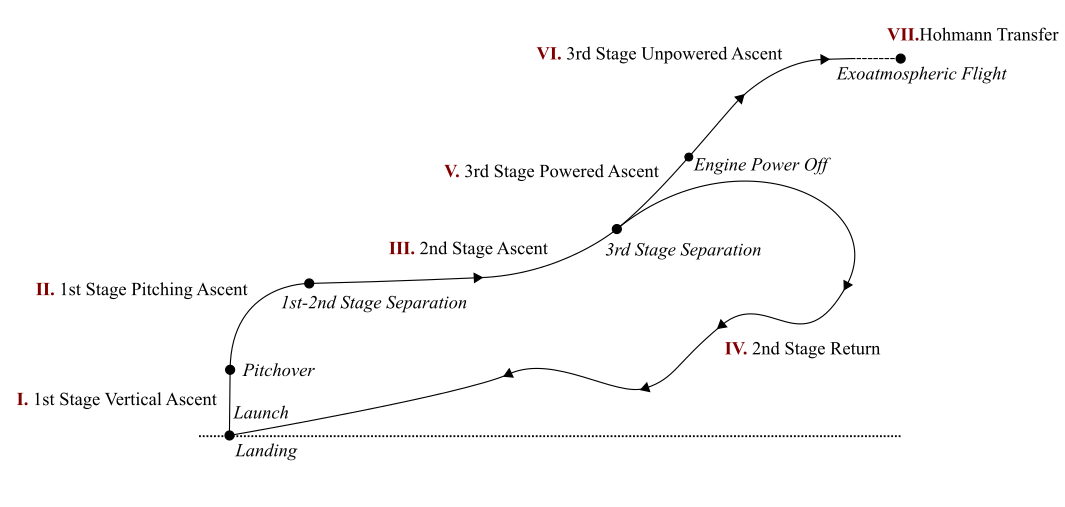
\includegraphics[width=1.\linewidth]{figures/4_LODESTAR/Traj}
 	\caption{Illustration of the segmented launch profile.}
 	\label{fig:Traj}
 \end{figure}
 
 To allow the trajectory profile to be formulated as an optimal control problem, the trajectory of the rocket-scramjet-rocket launch system has been broken down into the seven segments shown in Figure \ref{fig:Traj}. 
  The segments have been separated into two groups; controlled segments which take the form of phases within the optimal control problem; and segments without control which are either forward simulated at each iteration of the optimiser, or simulated externally to the optimal control problem. If the unpowered segments are simulated within the optimiser, they may be included in the cost and constraint functions of the optimisation problem.
  The unpowered segments are implemented in this way in order to increase computational efficiency and improve the convergence of the optimal control solver. 
  
 Segments \textcolor{red}{\rom{2}-\rom{5}} are controlled by various combinations of angle of attack, bank angle and throttle, and are implemented as the phases of the optimisation problem. These phases are; The 1st stage pitching ascent; the 2nd stage ascent; the 2nd stage return flight; and the 3rd stage powered ascent.
 Segments \textcolor{red}{\rom{1}},\textcolor{red}{\rom{6}} and \textcolor{red}{\rom{7}} are segments without direct control, which are simulated using forward time stepping methods. 
 These phases are; the pre-pitch segment of the first stage; the unpowered section of the third stage ascent; and the final Hohmann transfer to orbit. 
 Each segment is connected through a set of conditions, which ensure that the trajectory of the vehicle is continuous, and that the trajectory that is being simulated is the one that is intended. 
  The optimal control problem phases are connected through the use of initial and end discontinuity constraints on each phase to be coupled, ie $\textbf{x}_{f1} = \textbf{x}_{02}, t_{f1} = t_{02}$, while the forward simulated segments are simply initiated and terminated at set conditions. 
 The segment coupling conditions are described in Table \ref{tab:constraints}.






\begin{table}[H]


\begin{tabularx}{\linewidth}{|X|X|X|c|}
	\hline \textbf{Section} & Initial Conditions & End Conditions & Controlled \\ 
	\hline $1^{st}$ Stage Vertical Ascent (\textcolor{red}{\rom{1}}) & Launches from rest, at the predefined launch site. & Fly until pitchover conditions are met. & no \\ 
	\hline $1^{st}$ Stage Pitching Ascent (\textcolor{red}{\rom{2}}) & Start at pitchover conditions & -  & yes\\ 
	\hline $2^{nd}$ Stage Ascent (\textcolor{red}{\rom{3}}) & Must begin at $1^{st}$ stage pitching ascent end conditions. & - & yes\\ 
	\hline $2^{nd}$ Stage Return (\textcolor{red}{\rom{4}}) & Must begin at $2^{nd}$ stage ascent end conditions. & Must approach landing conditions at the initial launch site. & yes\\ 
	\hline $3^{rd}$ Stage Powered Ascent (\textcolor{red}{\rom{5}}) & Must begin at $2^{nd}$ stage ascent end conditions.  & Must produce exoatmospheric flight at the termination of stage \rom{6}.  & yes\\ 
	\hline $3^{rd}$ Stage Unpowered Ascent (\textcolor{red}{\rom{6}}) & Must begin at $3^{nd}$ stage powered ascent end conditions.  & Terminates when flight is parallel with Earth's surface.  & no\\ 
	\hline $3^{rd}$ Stage Hohmann Transfer (\textcolor{red}{\rom{7}}) & Must begin at $3^{rd}$ stage unpowered ascent end conditions. & Must attain prescribed orbit.  & no\\ 
	\hline 
	
\end{tabularx} 
\caption{Segment coupling conditions for combined trajectory optimisation.}
\label{tab:constraints}

\end{table}



\subsubsection{\textcolor{red}{\rom{1}.} First Stage Vertical Ascent}

LODESTAR optimises the ascent of the first stage rocket in two segments; pre and post-pitchover.
 These aerodynamics of flight during these segments are simulated using spline interpolation of the databases generated using the method described in Section \ref{sec:firststageaero}, and the engine properties are determined using linear pressure scaling as described in Section \ref{sec:firststage}. 
  
 The pre-pitchover phase is the segment of flight immediately after vertical launch. During this phase, the launch system continues vertically for a short time in order to clear the launch tower and stabilise the vehicle.        
The pre-pitchover section is not optimised, and is simulated externally to the optimisation to improve computational efficiency, and to allow the dynamics of the system to behave appropriately during the pitching ascent. During vertical flight, the heading angle (Equation \ref{eq:heading}) is meaningless, and vertical flight is allowed during the pitching ascent, the heading angle change rate can tend towards infinity, causing mathematical and scaling errors. Simulating this segment after the optimisation has been completed makes the starting mass and altitude of the first stage slightly variable, but this variation is negligible. 
The pitchover is defined to occur at 90m altitude and 15m/s velocity.
During the vertical launch the rocket is assumed to need no control, and is held at 0$^\circ$ angle of attack. 

\subsubsection{\textcolor{red}{\rom{2}.} First Stage Pitching Ascent}

At 90m altitude and 15m/s velocity, pitchover occurs. The pitchover is a very minor amount of instantaneous pitching (0.01$^\circ$) which is introduced in order to begin the pitching ascent, allowing the 6DOF dynamics of the vehicle to resolve correctly. 
The first stage pitching ascent trajectory is an angle of attack controlled phase in the optimisation routine, which is simulated from pitchover until second stage separation. Table \ref{tab:1ststagesetup} shows the optimisation setup of this phase. During this phase, the launch system is allowed to fly at negative angles of attack, to assist in pitching. The control of this phase is the second derivative of angle of attack. This is chosen as the control variable to assist in mitigating the first stage's sensitivity to angle of attack, ie. when the trajectory angle is near 90$^\circ$ and at low velocities, the effect of changes in angle of attack is very large. Using the second derivative of angle of attack as the control variable smooths the angle of attack change rate and improves the optimised solution. 
The initial fuel mass of the first stage rocket is unconstrained, as small variations in the initial fuel mass can have an important effect on the capabilities of the first stage. The fuel mass can influence the velocity achievable at first to second stage separation, as well as the rate at which the rocket is able to pitch, and consequentially, the altitude and flight path angle range of the first stage.
Allowing the initial fuel mass to vary increases the flexibility of the optimal control solver, though it is expected that the maximum allowable fuel mass will be used in most cases. 
The bounds on the latitude and longitude are chosen to cover the possible solution space, and are kept consistent across each phase to ensure that the position of the vehicle is not being unreasonably constrained between segments. The velocity constraints are chosen to cover the possible solution space, with the lower bound of 10m/s chosen to not allow the velocity to approach 0m/s, which produces singularities within the system dynamics. This velocity limit is true for all phases. 
The other bounds on the state dynamics are chosen to encompass the solution space, while not being overly expansive, to assist with the convergence and scaling of the optimal control solver, this is true for most of the bounds in all phases. 

\begin{table}[ht]
\centering
\begin{tabular}{|c|c|c|}
	\hline \textbf{Variable Group}  & \textbf{Associated Variables} & \textbf{Values}\\
	\hline Initial Constraints  & Velocity & 30m/s\\ & Altitude& 90m \\ & Latitude & $-12.16^\circ$ \\& Longitude & 136.75$^\circ$\\ & Trajectory Angle & 89.9$^\circ$\\ & Angle of Attack& 0$^\circ$\\
	\hline Terminal Constraints & $\textbf{x}_{f,\textrm{\rom{2}}} - \textbf{x}_{0,\textrm{\rom{3}}}$ & 0\\ & $t_{f,\textrm{\rom{2}}} - t_{0,\textrm{\rom{3}}}$ & 0\\
	\hline Path Constraints & Dynamic Pressure & 0kPa - 50kPa\\ 
		\hline Control Variables & $\ddot{\alpha}$ & $\pm0.029^\circ/s^2$\\ 
		\hline State Variables & Altitude & 0 - 30km\\ & Velocity& 10 - 3000m/s\\ & Trajectory Angle& $-5.7^\circ$ - $89.9^\circ$ \\   & Latitude& $\pm28.6^\circ$ \\  & Longitude& $114.6^\circ$ - $171.9^\circ$\\   & Heading Angle& $\pm360^\circ$\\  & Total Mass& 11453 - 29388kg \\  & Angle of Attack ($\alpha$)&  $-5^\circ$ - 0$^\circ$\\  & $\dot{\alpha}$& $\pm5.7^\circ/s$\\ 
	\hline 
\end{tabular} 

\caption{Optimisation setup of the first stage phase. }
\label{tab:1ststagesetup}
\end{table}



\subsection{\textcolor{red}{\rom{3}.} Second Stage Ascent Trajectory}
The second stage ascent phase consists of the acceleration of the SPARTAN scramjet-powered vehicle. 
The ascent trajectory of the SPARTAN is controlled using angle of attack and bank angle. The aerodynamics of the SPARTAN are interpolated from the engine on database developed as described in Sections \ref{sec:database} and \ref{sec:engine-on}. The engine properties are determined as described in Section \ref{sec:Propulsion}.
During the ascent, the engines are assumed to be operating at the maximum equivalence ratio at all times. This is 1 in most sections of the trajectory, except at low mach numbers where the possibility of unstart and choking necessitates a reduction in equivalence ratio. This trajectory is constrained to a maximum dynamic pressure of 50kPa, corresponding to the maximum structural limits of the vehicle. Aerodynamic and propulsion databases are generated as described in Sections \ref{sec:Propulsion} and \ref{sec:aero}. The lift and drag of the vehicle is interpolated from of the trimmed aerodynamics database and the propulsion is determined from interpolation of the C-REST database. 
The control variables are set as angle of attack and bank angle change rate. Using the derivatives of the angle of attack and bank angle as the control variables serves to smooth the angle of attack and bank angle by constraining the change rates to reasonable values. The angle of attack is constrained to 10$^\circ$, approximated as a reasonable upper bound to the angle of attack, and the limit to which the aerodynamic characteristics of the SPARTAN are modelled. The bank angle is constrained to a maximum of 90$^\circ$, as it is assumed that the SPARTAN is not able to invert. The bank angle is also constrained to positive values only (ie. that the heading angle may only increase) as the SPARTAN is launched from the ELA launch site at Nhulunbuy, and must be launched to the northeast or east to avoid overflying populated areas. 

A cost function can be included during this phase, when flying a constant dynamic pressure trajectory is desired. This cost function is configured as a quadratic cost function around 50kPa dynamic pressure, to ensure a smooth cost function, which goes to 0 at the target dynamic pressure. The cost function approaching 0 at the target dynamic pressure allows the cost function of payload mass (which is calculated during the third stage phases) to still be active, while prioritising flying constant dynamic pressure. This cost function is scaled by a constant scalar value, which has been tuned to ensure that the target dynamic pressure is matched closely during the acceleration of the SPARTAN, while still maximising payload-to-orbit during third stage optimisation. 


\begin{table}[ht]
	\centering
\begin{tabular}{|c|c|c|}
	\hline \textbf{Variable Group}  & \textbf{Associated Variables} & \textbf{Values}\\
	\hline Initial Constraints  & Fuel Mass & 1562kg\\ 
	\hline Terminal Constraints & Altitude & 0 - 45km\\ & Trajectory Angle& 0 - 15$^\circ$\\  & Bank Angle $\eta$& 0$^\circ$\\  & $\textbf{x}_{f,\textrm{\rom{3}}} - \textbf{x}_{0,\textrm{\rom{4}}}$ & 0\\ & $t_{f,\textrm{\rom{3}}} - t_{0,\textrm{\rom{4}}}$ & 0\\
	\hline Path Constraints & Dynamic Pressure& 0 - 50kPa\\ 
	\hline Target Cost & Dynamic Pressure$^*$ & $(q-50000)^2/50000$\\ 
			\hline Control Variables & $\dot{\alpha}$ &  $\pm0.5^\circ$/s\\  & $\dot{\eta}$ &  $\pm1^\circ$/s\\ 
			\hline State Variables & Altitude & 0 - 50km\\ & Velocity& 10 - 3000m/s\\ & Trajectory Angle& $-28.6^\circ$ - $15^\circ$\\   & Latitude&$\pm28.6^\circ$ \\  & Longitude& $114.6^\circ$ - $171.9^\circ$\\   & Heading Angle& $-240^\circ$ - $360^\circ$ \\  & Fuel Mass& 0 - 1562kg \\  & Angle of Attack ($\alpha$)&  0$^\circ$ - $10^\circ$ \\  & Bank Angle $\eta$& $-1^\circ$ - $90^\circ$ \\  
	\hline 
\end{tabular} 
\caption{Optimisation setup of the second stage ascent. $^*$ This is only used in the constant dynamic pressure simulation.}
\label{tab:SPARTANascentsetup}
\end{table}

\subsection{\textcolor{red}{\rom{4}.} Second Stage Return Trajectory}
After releasing the third stage rocket, the scramjet-powered second stage must return back to the initial launch site. During this return flight, the SPARTAN is able to use its engines if necessary to ensure that it is able to return successfully. The aerodynamics of the SPARTAN during fly-back are determined by interpolation of the engine-on and engine-off trimmed data sets described in Section \ref{sec:aero}. As the scramjet engines are throttled on, the aerodynamics are assumed to vary linearly between the aerodynamics calculated by the engine-off and engine-on datasets. 
During the fly-back, the SPARTAN cannot exceed its dynamic pressure limit of 50kPa. 
 The end state is constrained to a minimum of $-20^\circ$ trajectory angle, which is assumed to be an appropriate lower bound on the trajectory angle for approach to a landing strip. The altitude is constrained to less than 1km at the end point to ensure that the SPARTAN is approaching landing altitude.
 The velocity left unconstrained at the end point. Constraining the end velocity may over constrain the optimisation problem, and it is assumed that for a payload-to-orbit optimised trajectory the SPARTAN will end its return at a low velocity, so that the energy necessary for return is small. 
 
During the return, the C-REST engines are able to be throttled on and off. The throttle is set as a state variable, variable between 0 and 1, where 1 represents the maximum equivalence ratio at that point. The fuel mass flow rate is scaled linearly with the throttle:  
\begin{equation}
\dot{m}_{fuel} = \dot{m}_{fuel,max}throttle,
\end{equation}
and the thrust of the engine is assumed to scale linearly with the fuel mass flow rate. A control variable of throttle change rate is added, to smooth the throttle in the same was as angle of attack and bank angle. 

\begin{table}[ht]
	\centering
\begin{tabular}{|c|c|c|}
	\hline \textbf{Variable Group}  & \textbf{Associated Variables} & \textbf{Values}\\
	\hline Initial Constraints  & Bank Angle $\eta$& 0$^\circ$ \\ 
	\hline Terminal Constraints& Latitude & $-12.16^\circ$ \\& Longitude & 136.75$^\circ$\\
	\hline Path Constraints & Dynamic Pressure& 0 - 50kPa\\ 
				\hline Control Variables & $\dot{\alpha}$ &  $\pm0.5^\circ$/s\\  & $\dot{\eta}$ &  $\pm1^\circ$/s\\ & $\dot{Throttle}$& $\pm0.2$/s\\
				\hline State Variables& Altitude & 0 - 70km\\ & Velocity& 10 - 5000m/s\\ & Trajectory Angle& $\pm80^\circ$\\    & Latitude&$\pm28.6^\circ$ \\  & Longitude& $114.6^\circ$ - $171.9^\circ$\\   & Heading Angle& $60^\circ$ - $500^\circ$ \\  & Fuel Mass& 0kg - 500kg\\  & Angle of Attack ($\alpha$)&  0$^\circ$ - 10$^\circ$\\  & Bank Angle ($\eta$)& $0^\circ$ - 90$^\circ$\\  & Throttle & 0 - 1 \\ 
	\hline 
\end{tabular} 
\caption{Optimisation setup of the second stage return.}

\end{table}

\subsection{\textcolor{red}{\rom{5}.} Third Stage Powered Ascent}
The trajectory of the third stage rocket is separated into the powered and unpowered phases of ascent.
During the powered ascent phase, the third stage is manoeuvred out of the atmosphere using one continuous burn of the Kestrel engine. 
 The powered phase is controlled using angle of attack, and trimmed using thrust vectoring of the engine, as described in Section \ref{sec:thrustvectoring}. The aerodynamics of the third stage are determined using interpolation of the aerodynamic dataset developed as described in Section \ref{sec:thirdstageaero}.

The third stage rocket is constrained to an angle of attack of less than 20$^\circ$. This is assumed to be the maximum controllable angle of attack possible for the third stage rocket.   
Additionally, a maximum normal force restriction is placed on the third stage, to limit the angle of attack of the third stage by the normal force on the vehicle. However, as a detailed structural study of the third stage has not been conducted, the maximum allowable normal force on the third stage is not known.
For consistency, the maximum allowable normal force was calculated from the conditions of previous studies. Previous studies flew the third stage rocket at a constant 10$^\circ$ angle of attack, and initially released the rocket at 50kPa[CITEXX]. 
It is assumed that this condition of 10$^\circ$ angle of attack and 50kpa dynamic pressure produces the maximum allowable normal force to prevent the rocket from being released into an environment which could exceed its structural limitations. The maximum allowable normal force is calculated at the release Mach number, and is set as a path constraint. 

The end angle of attack is constrained to 0$^\circ$, as the angle of attack will not be able to be controlled during the unpowered ascent. 
The other terminal constraints of this phase correspond to end constraints imposed after the third stage unpowered ascent has been simulated. The altitude at the end of the unpowered ascent (Phase \rom{6}) is constrained to a lower limit of 90km, in order to ensure that the circularisation burn is exoatmospheric. The final heading angle is also constrained at this point, so that the orbit of the third stage is circularised into the correct inclination for sun synchronous orbit. 

\begin{table}[ht]
	\centering
\begin{tabular}{|c|c|c|}
\hline \textbf{Variable Group}  & \textbf{Associated Variables} & \textbf{Values}\\	\hline Initial Constraints  & Total Mass & 3300kg\\  & $\textbf{x}_{f,\textrm{\rom{3}}} - \textbf{x}_{0,\textrm{\rom{5}}}$ & 0\\ & $t_{f,\textrm{\rom{3}}} - t_{0,\textrm{\rom{5}}}$ & 0\\
	\hline Terminal Constraints & Alt$_{f,\textrm{\rom{6}}}$ & $\geq$90km\\ & Heading Angle, $\zeta_{f,\textrm{\rom{6}}}$ & 97.64$^\circ$\\  & Angle of Attack ($\alpha$) & 0$^\circ$\\
	\hline Path Constraints & Angle of Attack ($\alpha$) & Maximum $F_N$\\  & Thrust Vector Angle & $\pm8^\circ$\\ 
	\hline Target Cost & Payload-to-Orbit & Payload Calculated in Phase \rom{7}\\ 
				\hline Control Variables & $\dot{\alpha}$ & $\pm1^\circ$\\ 
				\hline State Variables & Altitude & 30 - 84km\\ & Velocity& 10 - 8000m/s\\ & Trajectory Angle& $-5^\circ$ - 30$^\circ$ \\   & Latitude&$\pm28.6^\circ$ \\   & Heading Angle& $80^\circ$ - 120$^\circ$\\  & Total Mass& 0kg - 3300kg \\  & Angle of Attack ($\alpha$)&  $-5^\circ$ - 0$^\circ$\\ 
	\hline 
\end{tabular} 
\caption{Optimisation setup of the third stage powered ascent.}
\end{table}

\subsection{\textcolor{red}{\rom{6}.} Third Stage Unpowered Ascent}
After the burn of the Kestrel engine is complete, the engine is cut and the third stage coasts to a point where it is able to be circularised into a low orbit. 
The unpowered phase of the ascent is not controlled. After the engine is cut, the third stage does not have sufficient aerodynamic control to manoeuvre, and the trajectory of the third stage is a coast at 0$^\circ$ angle of attack. The trajectory of the third stage rocket is only directly optimised during the powered section of its trajectory, the unpowered section of the trajectory is simulated from the end of the controlled section of the trajectory, using a second order Taylor series approximation. This integration ceases when the flight path angle reaches 0$^{\circ}$.
During this phase, the heat shield is released once the rocket has reached a dynamic pressure of 10Pa, where it is assumed that atmospheric effects will have ceased to have a major thermal effect.  As the third stage is required to deliver the payload into heliosynchronous orbit, the third stage must achieve an inclination of 97.63$^\circ$ at the end of this phase[CITEXX]. These terminal constraints are implemented in Phase \rom{5}.



\subsection{\textcolor{red}{\rom{7}.} Hohmann Transfer}
After the rocket has attained exoatmospheric flight parallel to the Earth's surface, a circularisation burn is performed. This circularisation burn takes the third stage rocket into low orbit around the Earth. 
However, in order to reach a heliosynchronous orbit of 567km, the orbit of the third stage rocket must be raised. 
To this end, the final manoeuvre performed by the third stage rocket is a Hohmann transfer. A Hohmann transfer is the most fuel efficient way to raise a spacecraft from one circular orbit to another[CITEXX]. 
\begin{figure}
\centering
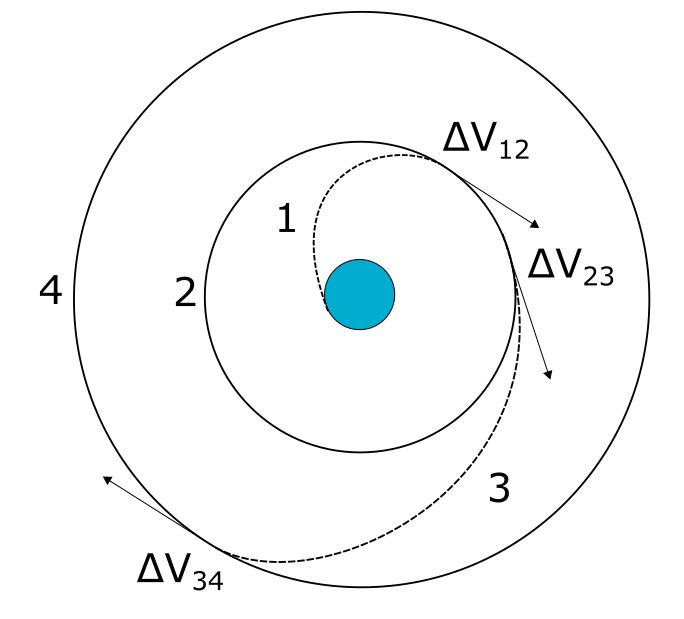
\includegraphics[width=0.7\linewidth]{figures/4_LODESTAR/Hohmann}
\caption{The Hohmann transfer manoeuvre.}
\label{fig:Hohmann}
\end{figure}
The orbit of the third stage is first circularised into a low orbit:
\begin{equation}
\Delta V_{12} = \sqrt{\dfrac{\mu}{r_2}} - V_1.
\end{equation}
Following circularisation, the third stage engine is reignited (or remains ignited) and the third stage manoeuvres into an appropriate elliptical orbit: 
\begin{equation}
\Delta V_{23} = \sqrt{\dfrac{\mu}{r_2}} \left( \sqrt{\dfrac{2r_4}{r_2 + r_4}} -1 \right).
\end{equation}
At the apogee of the transfer orbit, corresponding to the desired orbital radius, an insertion burn is performed, and the orbit is circularised:
\begin{equation}
\Delta V_{34} = \sqrt{\dfrac{\mu}{r_4}} \left(1- \sqrt{\dfrac{2r_2}{r_2 + r_4}}  \right).
\end{equation}
At this point, the payload is separated from the third stage rocket. 

The mass of the third stage rocket after each burn is calculated using the Tsiolkovsky rocket equation:
\begin{equation}
m_2 = \frac{m_{1f}}{\exp^{\frac{V_{12}}{I_{SP} \cdot g_0}}}
\end{equation}
\begin{equation}
m_3 = \frac{m_{2}}{\exp^{\frac{V_{23}}{I_{SP} \cdot g_0}}}
\end{equation}
\begin{equation}
m_4 = \frac{m_{3}}{\exp^{\frac{V_{34}}{I_{SP} \cdot g_0}}}
\end{equation}
Finally, the payload-to-orbit is determined by removing the structural mass from the total mass of the vehicle at the end of the Hohmann transfer. The remaining mass is taken to be the payload-to-orbit capability of the vehicle.
\begin{equation}
m_{payload} = m_4 - m_{struct}
\end{equation}







\section{Optimal Solution Analysis}\label{sec:verification}

LODESTAR provides the capacity to analyse the optimal solution provided by the pseudospectral method solver to assist in determining whether the pseudospectral method solver has converged close to an optimal solution of the nonlinear programming problem. It is particularly useful to verify that the optimality and constraint tolerances that have been chosen are sufficiently small, or to check whether the pseudospectral method solver has approached an optimal solution in the case that the defined tolerances are not able to be reached.   
Checking the solution is achieved through the examination of five key metrics; the IPOPT constraint violation and dual infeasibility parameters; the Hamiltonian necessary condition for optimality; the state derivatives; and finally a forward simulation. 

The first metrics to be checked are the IPOPT constraint violation ($inf\textrm{-}pr$) and dual infeasibility parameter ($inf\textrm{-}du$)\cite{Kawajir2010}. The constraint violation parameter is a measure of the infinity-norm ($L_\infty\textrm{-}norm$) of the constraints of the problem\cite{Kawajir2010}. This factor must be suitably small in order to indicate that the constraints of the problem have been met. While the permissible magnitude of this factor changes with each individual problem, it is always desirable for this factor to be as small as possible. The dual infeasibility provides an indication of the optimality of the solution. A low dual infeasibility indicates that the solution is dual feasible and is likely to have approached an optimal solution. A dual feasible solution indicates that the dual problem is at least a lower bound on the optimal solution, $p^\star$, ie. $p^\star \geq g(\lambda,v)$. For more details on duality see Reference \cite{Hindi2006}.
 Again, the magnitude of this value is variable with each problem, though as a problem becomes more complex, the ability to converge towards an optimal solution diminishes. It should generally be observable that the $inf\textrm{-}du$ term is decreasing by multiple orders of magnitude and is stable at the completion of optimisation for a solution to be approaching optimality. In this study it is accepted that a given solution may not approach the global optimum, and multiple solutions are calculated to mitigate the error caused by the problem complexity, with the 'most optimal' solution selected. 


The Hamiltonian of the optimal control problem is defined as 
\begin{equation}
H(x(t),u(t),\lambda(t),t) = \lambda^T(t)f(x(t),u(t)) + L(x(t),u(t)).
\end{equation}
The Hamiltonian of the optimal control problem is investigated as a partial verification that the first order necessary conditions hold. Due to the unconstrained end time of the trajectory problems, $H\equiv 0 $ \cite{Pucci2007}. 
This is calculated using LODESTAR and the Hamiltonian condition is able to be verified. A sufficiently small Hamiltonian indicates that the end solution is likely to have approached an optimal solution.


The pseudospectral method considers the dynamics of the system as constraints on the optimal control problem, and solves across the entire trajectory simultaneously. This causes the physical system dynamics to have an associated margin of error, ie. $\dot{x} = f(x)$ will only hold to a certain degree of accuracy. For a well converged solution, this margin of error will be negligibly small, and the dynamics of the system will be consistent with realistic Newtonian dynamics. However, when the problem is not well converged, the dynamics of the system may have a large error.
A check is performed on each state to affirm that the derivative of the approximated state is equal to the derivative supplied by the vehicle model. This checks that the solver has converged to a solution which satisfies the vehicle dynamics at each individual node. 
The state feasibility of the solution is checked through a comparison of the state derivatives, $\dot{x} = f(x,u)$. $\dot{x}$ is first determined through numerical differentiation of the state variables over the solution time, differentiated at the node points created by GPOPS-2. Then $f(x,u)$ is determined using the dynamics of the system and vehicle model, in the same way that $f(x,u)$ is input to the pseudospectral solver. Examination of the error between the 'expected' state derivatives, and the numerical approximation of the derivatives, $\dot{x} - f(x,u)$, allows the accuracy of the system dynamics to be assessed. 



 The final verification check is a full forward simulation. This forward simulation starts at the initial conditions prescribed by the pseudospectral method solver, and propagates the dynamics of the system forward in time using the Runge-Kutta method, through Matlab's ODE45 function. The forward simulation uses the optimised control variables as the only input. 
This checks that the flight path will follow the path computed by GPOPS-2, using only the calculated control inputs. This is the most complete test of the optimal solution. However, in some cases calculating a forward solution may be problematic. The pseudospectral method has a limited number of nodes, potentially spread across relatively large time steps. Due to the high accuracy of the polynomial approximation, the pseudospectral method is able to maintain accuracy over large time steps. However, a forward simulation necessarily has less accuracy than the spectral method, and may interpolate differently when applied to the optimal solution, causing minor deviations. These variations are usually negligibly small, however, this is problematic during the return phase, due to the way the throttling of the engines is modelled, ie. the specific impulse of the engines is set to 0 under Mach 5 or 20kPa inlet conditions during the optimisation process. As the engines are often throttled close to the minimum operable conditions, these restrictions can intensify the effects of otherwise minor deviations in the forward simulation.
 For this reason, the forward simulation of the return stage is split into three segments, with divisions at 1/6th and 1/3rd of the total trajectory length, chosen to separate the first major 'skip' and bank, and split the 'skipping' section of the trajectory. A forward simulation is initiated at each of these segments, mitigating some of the effects of the engines throttling on and off in the forward simulation. 
Splitting the forward simulation allows the forward simulation of the return stage to be assessed without the effects of the throttle model having an unreasonably large effect. 


\section{The Optimisation Process}

Figure \ref{fig:AscentFlowchart} shows the flow chart of the optimisation process, including the external simulation modules. The main process is run multiple times, with varying initial guesses, in order to be able to select the most converged solution. This process is parallelised, with green and red arrows in Figure \ref{fig:AscentFlowchart} indicating the initiation and termination of the parallel loop respectively. 


\begin{landscape}% Landscape page
	\begin{figure}[ht]
		\centering
		\includegraphics[width=0.98\linewidth]{"figures/4_LODESTAR/Ascent Flowchart"}
		\caption{The process of the rocket-scramjet-rocket trajectory optimisation. Relevant sections are indicated in square brackets at each process step.}
		\label{fig:AscentFlowchart}
	\end{figure} 
\end{landscape}

